\begin{figure}[hp]
    \centering
    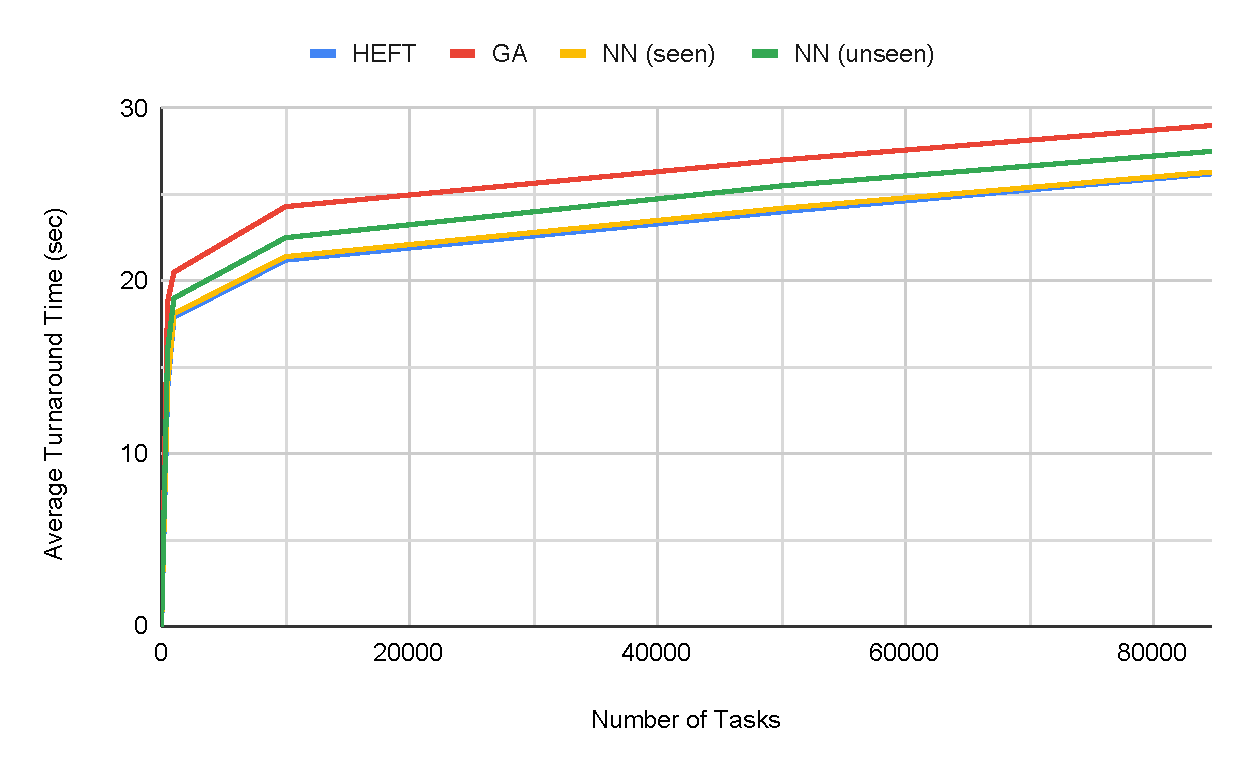
\includegraphics[width=0.45\textwidth]{diagrams/ta_chart}
    \caption{Average turnaround time produced from the three discussed schedulers at different input sizes.}
    \label{fig:ta_chart}
\end{figure}

\subsection{Scheduling Performance}

Fig.\ref{fig:ta_chart} shows the scheduling performance of different scheduling methods at different input sizes. The proposed network shows almost the same average turnaround time as HEFT algorithm for the seen data during training. However, for unseen data, the network shows slightly more poor performance than HEFT, but still better than that of genetic algorithms. 

These results refer to the network ability to learn a good representation to the input machines and scheduling problem. The network performance degrades with high input sizes, as it's approximating HEFT, which is basically a greedy algorithm and prone to failure at complex situations. Genetic algorithms shows similar behaviour too, due to large population size.

\subsection{Execution Time}
\begin{table}
  \caption{Time comparison between the three discussed schedulers at different input sizes. Time measured in seconds.}
  \label{tab:exec_time}
  \centering
  \begin{tabular}{l l l l}
    \toprule
    Input Size & HEFT & GA & NN \\
    \midrule
    486	& 31.5 & 67.5 & 0.125 \\
    10000 & 305.5 & 602.5 & 0.125 \\
    84654 & 670.0 & 3967.0 & 0.125 \\
    \bottomrule
  \end{tabular}
\end{table}

The main advantage of using neural networks is constant inference time. Once the network is trained, it takes a static execution time in inference, as it's a simple feedforward process. Table \ref{tab:exec_time} shows the execution time of the discussed schedulers at 3 different input sizes. These number are produced running on \emph{Intel i5-6600K}. 

We can see that the network consumes constant time in inference with different input sizes. This is because the network is trained on the maximum input length. However, HEFT and genetic algorithms execution time increases with input size. GA time increases more rapidly than HEFT, as it's a recursive optimization method but HEFT is a greedy-based method.

\subsection{Results Discussion}
The previous results show that neural networks can approximate a scheduling algorithm for heterogeneous distributed systems, resulting in a significantly-good performance and fast execution. The proposed network can perform well, even on unseen data it can produce efficient schedules.

However, this comes with a drawback of static scenarios. The neural network is trained with fixed input size, which is the maximum number of tasks, in our case. At inference time, the input to the network can't exceed that number. So, we have to define the maximum number of tasks to be scheduled, as well as the maximum number of resources. Moreover, the scheduling scenario for the proposed network should be static, where all available tasks should be known before the scheduler starts. 

This gives neural networks a great potential to be a good task scheduler in static scenarios, where the maximum number of tasks and resources are known. However, in other dynamic scenarios, neural networks might not help much. 